\documentclass[reqno,a4paper,12pt]{amsart}

\usepackage{amsmath,amssymb,amsthm,geometry,xcolor,soul,graphicx}
\usepackage{titlesec}
\usepackage{enumerate}
\usepackage{lipsum}
\usepackage{listings}
%\RequirePackage[most]{tcolorbox}
\usepackage{braket}
\allowdisplaybreaks[4] %align公式跨页
\usepackage{xeCJK}
\setCJKmainfont[AutoFakeBold = true]{Kai}
\geometry{left=0.7in, right=0.7in, top=1in, bottom=1in}

\renewcommand{\baselinestretch}{1.3}

\title{介观物理第四次作业}
\author{董建宇 ~~ 202328000807038}

\begin{document}

\maketitle
\titleformat{\section}[hang]{\small}{\thesection}{0.8em}{}{}
\titleformat{\subsection}[hang]{\small}{\thesubsection}{0.8em}{}{}

\textbf{Problem I.10} Derive the diamagnetic part in Eq. (68).
\begin{equation}
	\tag{68}\sigma_{\alpha\beta}(\omega) = \frac{1}{i\omega} \left[ \Pi_{\alpha\beta}(\omega) - \frac{ne^2}{m} \delta_{\alpha\beta} \right]. 
\end{equation}

\begin{proof}
抗磁电流密度为:
\[
	\mathbf{j}_D = -\frac{e^2}{m}\mathbf{A}(\mathbf{r}) \rho(\mathbf{r}).
\]

%利用Kubo公式计算响应函数如下:
%\begin{align*}
%	&i\int_{-\infty}^t dt' e^{i\omega(t-t')} \bra{0} [j_{D\alpha}(t), j_{D\beta}(t')] \ket{0} \\
%	=&
%\end{align*}
可以将电子密度近似为$n = \langle \rho(\mathbf{r}) \rangle$,则有:
\[
	\mathbf{j}_D = -\frac{ne^2}{m}\mathbf{A}(\mathbf{r}).
\]

利用
\[
	\mathbf{E}(t) = -\frac{\partial \mathbf{A}(t)}{\partial t}; \ \ \mathbf{E}(\omega) = i\omega \mathbf{A}(\omega).
\]

可以得到:
\[
	\mathbf{j}_D(\omega) = -\frac{ne^2}{m} \frac{1}{i\omega} \mathbf{E}(\omega).
\]

写成分量形式,即:
\[
	j_{D\alpha}(\omega) = -\frac{1}{i\omega} \frac{ne^2}{m} \delta_{\alpha\beta} E_{\beta}(\omega).
\]

即响应函数抗磁项为:
\[
	{\sigma_{\alpha\beta}}_D = -\frac{1}{i\omega} \frac{ne^2}{m} \delta_{\alpha\beta}.
\]

\end{proof}


\textbf{Problem I.11} Write down the Kramers-Kronig relation for $\sigma_1(\omega)$ and $\sigma_2(\omega)$.

\begin{proof}
\[
\left\{
\begin{aligned}
	&\sigma_1(\omega) = \int_{-\infty}^\infty \frac{d\omega'}{\pi} \sigma_2(\omega') P \frac{1}{\omega'-\omega}; \\
	&\sigma_2(\omega) = -\int_{-\infty}^\infty \frac{d\omega'}{\pi} \sigma_1(\omega') P \frac{1}{\omega'-\omega}.
\end{aligned}
\right.
\]
\end{proof}


\textbf{Problem I.12} Verify Eq. (70b). Hint: Use Eq. (68).
\[
	\sigma(\omega\pm i0^+) = \pm\sigma_1(\omega) + i\sigma_2(\omega). \tag{70b}
\]

\begin{proof}
对于直流电,$\omega = 0$,电导是一个有限值,即
\[
	\Pi_{\alpha\beta}(\mathbf{q}=0, \omega=0) = i\int_{-\infty}^t dt' \langle [j_{P\alpha}(t), j_{P\beta}(t')] \rangle = \frac{ne^2}{m}\delta_{\alpha\beta}
\]

即有$\langle [j_{P\alpha}(t), j_{P\beta}(t')] \rangle$为纯虚数。考虑电流电流耦合项拆分成实部和虚部$\Pi_{\alpha\beta}(\omega) = \Pi_{\alpha\beta}^{(1)}(\omega) + i\Pi_{\alpha\beta}^{(2)}(\omega)$:
\begin{align*}
	\Pi_{\alpha\beta}(\omega) =& i \int_{-\infty}^t dt' e^{i\omega(t-t')} \langle [j_{P\alpha}(t), j_{P\beta}(t')] \rangle \\
	=& i \int_{-\infty}^t dt' [\cos\omega(t-t') + i\sin\omega(t-t')] \langle [j_{P\alpha}(t), j_{P\beta}(t')] \rangle \\
	=& i\int_{-\infty}^t dt' \cos[\omega(t-t')] \langle [j_{P\alpha}(t), j_{P\beta}(t')] \rangle - \int_{-\infty}^t dt' \sin[\omega(t-t')] \langle [j_{P\alpha}(t), j_{P\beta}(t')] \rangle.
\end{align*}

即有:
\[
\left\{\begin{aligned}
	\Pi_{\alpha\beta}^{(1)}(\omega) =& i\int_{-\infty}^t dt' \cos[\omega(t-t')] \langle [j_{P\alpha}(t), j_{P\beta}(t')] \rangle; \\
	\Pi_{\alpha\beta}^{(2)}(\omega) =& i\int_{-\infty}^t dt' \sin[\omega(t-t')] \langle [j_{P\alpha}(t), j_{P\beta}(t')] \rangle.
\end{aligned} \right.
\]



从而可以得到电导率的实部和虚部分别为:
\[
\left\{ \begin{aligned}
	\sigma_1(\omega) =& \frac{1}{\omega}\Pi^{(2)}_{\alpha\beta}(\omega) = \frac{i}{\omega} \int_{-\infty}^t dt' \sin[\omega(t-t')] \langle [j_{P\alpha}(t), j_{P\beta}(t')] \rangle; \\
	\sigma_2(\omega) =& \frac{1}{\omega} \left[ \frac{ne^2}{m}\delta_{\alpha\beta} - \Pi^{(1)}_{\alpha\beta} \right] = \frac{1}{\omega} \left[ \frac{ne^2}{m}\delta_{\alpha\beta} - i\int_{-\infty}^t dt' \cos[\omega(t-t')] \langle [j_{P\alpha}(t), j_{P\beta}(t')] \rangle \right].
\end{aligned} \right. 
\]

可以计算:
\[
\begin{aligned}
	\sin[(\omega+i0^+)(t-t')] =& \sin[\omega(t-t')]\cosh[0^+(t-t')] + i\cos[\omega(t-t')]\sinh[0^+(t-t')]; \\
	\cos[(\omega+i0^+)(t-t')] =& \cos[\omega(t-t')]\cosh[0^+(t-t')] - i\sin[\omega(t-t')]\sinh[0^+(t-t')].
\end{aligned}
\]

在原始电导率表达式中,考虑$\sigma(\omega\pm0^+)$如下:
\begin{align*}
	\sigma_{\alpha\beta}(\omega+i0^+) =& \frac{1}{i(\omega+i0^+)} \left[ -\frac{ne^2}{m}\delta_{\alpha\beta} + i\int_{-\infty}^t dt' e^{i(\omega+i0^+)(t-t')} \langle [j_{P\alpha}(t), j_{P\beta}(t')] \rangle \right] \\
	=& \frac{1}{i\omega-0^+} \left[ -\frac{ne^2}{m}\delta_{\alpha\beta} + i\int_{-\infty}^t dt' e^{i\omega(t-t')} e^{-0^+(t-t')} \langle [j_{P\alpha}(t), j_{P\beta}(t')] \rangle \right] \\
	=& -\frac{i\omega+0^+}{\omega^2} \left[ -\frac{ne^2}{m}\delta_{\alpha\beta} + i\int_{-\infty}^t dt' \cos[\omega(t-t')] e^{-0^+(t-t')} \langle [j_{P\alpha}(t), j_{P\beta}(t')] \rangle \right] \\
	&+ \frac{i\omega+0^+}{\omega^2} \int_{-\infty}^t dt' \sin[\omega(t-t')] e^{-0^+(t-t')} \langle [j_{P\alpha}(t), j_{P\beta}(t')] \rangle; \\
	\sigma_{\alpha\beta}(\omega-i0^+) =& \frac{1}{i(\omega-i0^+)} \left[ -\frac{ne^2}{m}\delta_{\alpha\beta} + i\int_{-\infty}^t dt' e^{i(\omega-i0^+)(t-t')} \langle [j_{P\alpha}(t), j_{P\beta}(t')] \rangle \right]	\\
	=& \frac{1}{i\omega+0^+} \left[ -\frac{ne^2}{m}\delta_{\alpha\beta} + i\int_{-\infty}^t dt' e^{i\omega(t-t')} e^{0^+(t-t')} \langle [j_{P\alpha}(t), j_{P\beta}(t')] \rangle \right] \\
	=& -\frac{i\omega-0^+}{\omega^2} \left[ -\frac{ne^2}{m}\delta_{\alpha\beta} + i\int_{-\infty}^t dt' \cos[\omega(t-t')] e^{0^+(t-t')} \langle [j_{P\alpha}(t), j_{P\beta}(t')] \rangle \right] \\
	&+ \frac{i\omega+0^+}{\omega^2} \int_{-\infty}^t dt' \sin[\omega(t-t')] e^{0^+(t-t')} \langle [j_{P\alpha}(t), j_{P\beta}(t')] \rangle; \\
\end{align*}

\end{proof}


\textbf{Problem I.13} Derive Eq. (79) using Eq. (70b). Hint: Consider a contour deformation as follows:
\begin{center}
	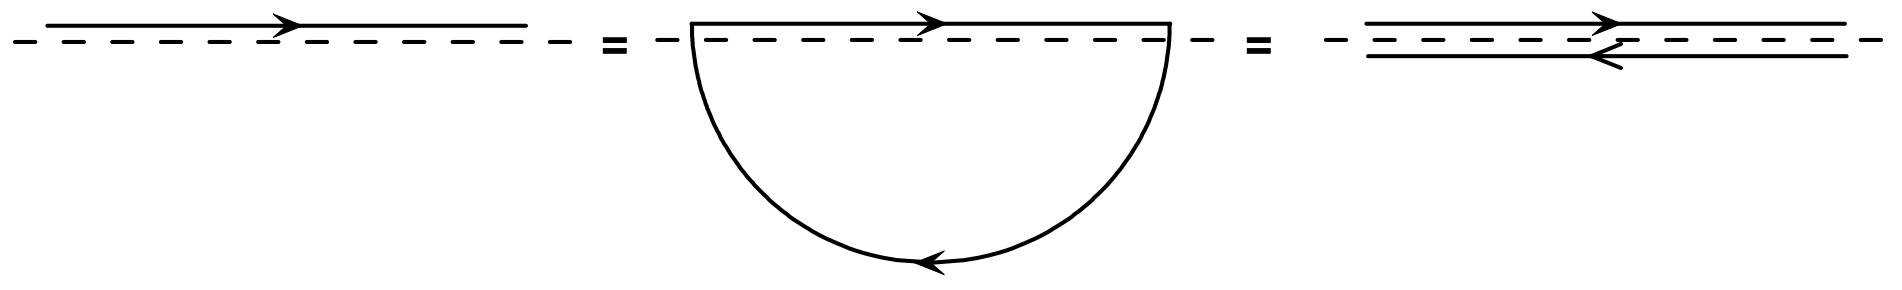
\includegraphics[scale = 0.2]{homework04_P13.jpeg}
\end{center}
\[
	\sigma(\omega\pm i0^+) = \pm \sigma_1(\omega) + i\sigma_2(\omega). \tag{70b}
\]

\[
	\frac{ne^2}{m} = \int_{-\infty}^\infty \frac{d\omega}{2\pi} e^{-i\omega 0^+} \sigma(\omega) = \int_{-\infty}^\infty \frac{d\omega}{2\pi} [\sigma_1(\omega) + i\sigma_2(\omega)] = \int_0^\infty \frac{d\omega}{\pi} \sigma_1(\omega). \tag{79}
\]
%Do the frequency sum in the last line of Eq. (85).
%\[
%	-\frac{1}{\beta} \sum_m \mathcal{G}^{(0)}(\mathbf{p}+\mathbf{q}, i\nu_m) \mathcal{G}^{(0)}(\mathbf{p}, i\nu_m + i\omega_n) = -\frac{n_F(\xi_{\mathbf{p}+\mathbf{q}}) - n_F(\xi_\mathbf{p})}{i\omega_n + \xi_{\mathbf{p}+\mathbf{q}} - \xi_\mathbf{p}}. \tag{85}
%\]

\begin{proof}
注意到由于复平面下半平面无穷远处模收敛,所以从$-\infty$到$\infty$的积分可以拓展到复平面下半平面,形成闭合回路积分。下半平面无穷远处的积分,可以连续变换至位于实轴下方无穷小距离处从正无穷到负无穷的积分。即:
%由于$\sigma(\omega) = \frac{ne^2}{m} \frac{1}{\tau^{-1}-i\omega}$的一阶奇点为$\omega = $
\begin{align*}
	\int_{-\infty}^\infty \frac{d\omega}{2\pi} e^{-i\omega 0^+} \sigma(\omega) =& \oint \frac{d\omega}{2\pi} e^{-i\omega 0^+} \sigma(\omega) \\
	=& \int_{-\infty}^\infty \frac{d\omega}{2\pi} \sigma(\omega+i0^+) + \int_{\infty}^{-\infty}\frac{d\omega}{2\pi} \sigma(\omega-i0^+) \\
	=& \int_{-\infty}^\infty \frac{d\omega}{2\pi} [\sigma(\omega+i0^+) - \sigma(\omega-i0^+)] \\
	=& \int_{-\infty}^\infty \frac{d\omega}{\pi} \sigma_1(\omega) \\
	=& 2\int_0^\infty \frac{d\omega}{\pi} \sigma_1(\omega) \\
	=& \frac{ne^2}{m}.
\end{align*}

其中,利用了
\[
	\sigma(\omega+i0^+) - \sigma(\omega-i0^+) = \sigma_1(\omega) + i\sigma_2(\omega) - [-\sigma_1(\omega) + i\sigma_2(\omega)] = 2\sigma_1(\omega).
\]
\end{proof}


\end{document}